\begin{figure}[!htbp]
  \centering 
\begin{minipage}[b]{0.45\textwidth}
    \centering
    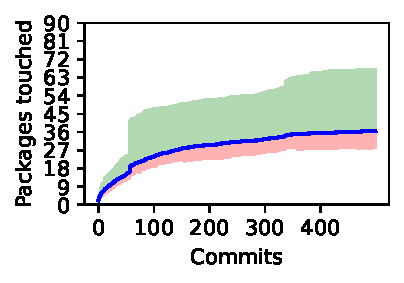
\includegraphics[width=\textwidth]{ sections/results/packages/time_series_components_touched.packages.all.founders.commits_500.pdf }
    \vskip 5pt
    {\small Packages for All founders (n=34 \& $\mu$=24.94)}
    \label{ figure.58.20000000000019 }
\end{minipage}%
\hfill
\begin{minipage}[b]{0.45\textwidth}
    \centering
    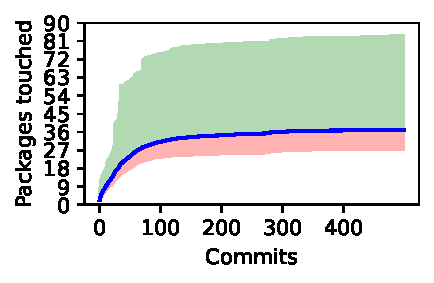
\includegraphics[width=\textwidth]{ sections/results/packages/time_series_components_touched.packages.all.joiners.commits_500.pdf }
    \vskip 5pt
    {\small Packages for All joiners (n=203 \& $\mu$=27.84)}
    \label{ figure.58.30000000000019 }
\end{minipage}%
\hfill
\newpage 
\begin{minipage}[b]{0.45\textwidth}
    \centering
    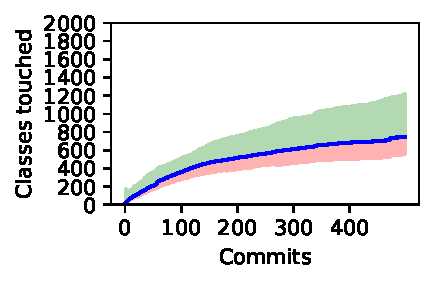
\includegraphics[width=\textwidth]{ sections/results/classes/time_series_components_touched.classes.all.founders.commits_500.pdf }
    \vskip 5pt
    {\small Classes for All founders (n=34 \& $\mu$=746.59)}
    \label{ figure.66.40000000000018 }
\end{minipage}%
\hfill
\begin{minipage}[b]{0.45\textwidth}
    \centering
    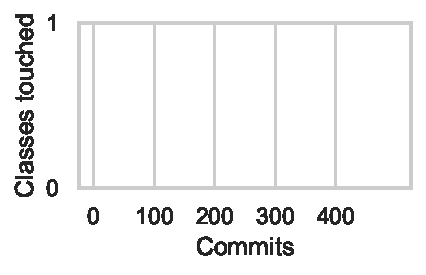
\includegraphics[width=\textwidth]{ sections/results/classes/time_series_components_touched.classes.all.joiners.commits_500.pdf }
    \vskip 5pt
    {\small Classes for All joiners (n=203 \& $\mu$=442.33)}
    \label{ figure.66.50000000000017 }
\end{minipage}%
\hfill
\newpage 
\begin{minipage}[b]{0.45\textwidth}
    \centering
    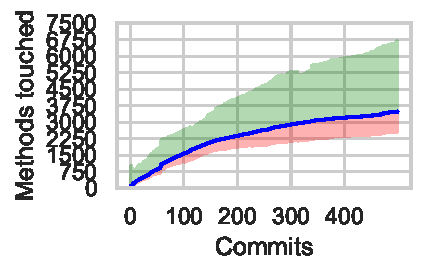
\includegraphics[width=\textwidth]{ sections/results/methods/time_series_components_touched.methods.all.founders.commits_500.pdf }
    \vskip 5pt
    {\small Methods for All founders (n=34 \& $\mu$=3095.18)}
    \label{ figure.73.60000000000005 }
\end{minipage}%
\hfill
\begin{minipage}[b]{0.45\textwidth}
    \centering
    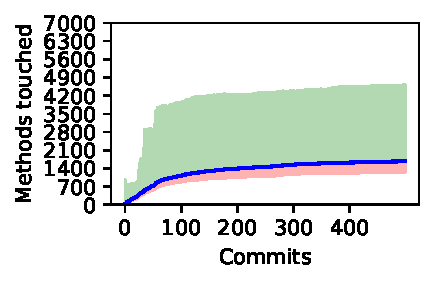
\includegraphics[width=\textwidth]{ sections/results/methods/time_series_components_touched.methods.all.joiners.commits_500.pdf }
    \vskip 5pt
    {\small Methods for All joiners (n=203 \& $\mu$=1672.84)}
    \label{ figure.73.70000000000005 }
\end{minipage}%
\hfill
\caption{A time series for the all commits, excluding transient, with the average mean (blue line), all components touched (y-axis) against the number of commits (x-axis) for two (2) developer categories. Green is the standard deviation above the mean, and pink is the standard deviation below the mean.}\end{figure}
\newpage 
\newpage 
